\documentclass[a4j]{ujarticle}
% \documentclass[a4j]{jarticle}
\renewcommand{\baselinestretch}{0.85}
\usepackage[top=1.5cm, bottom=1.5cm, left=1.5cm, right=1.5cm]{geometry}
\usepackage{xcolor}
\usepackage[dvipdfmx]{graphicx, hyperref}
\usepackage{listings}
\usepackage{multirow}
\usepackage{siunitx}
\usepackage{subfig}
\usepackage{url}
\usepackage{listings}

\colorlet{punct}{red!60!black}
\definecolor{background}{HTML}{EEEEEE}
\definecolor{delim}{RGB}{20,105,176}
\colorlet{numb}{magenta!60!black}

\newcommand{\Sref}[1]{\mbox{\ref{sec:#1}}}
\newcommand{\Tref}[1]{\mbox{表\ref{tab:#1}}}
\newcommand{\Eref}[1]{\mbox{式(\ref{eq:#1})}}
\newcommand{\Fref}[1]{\mbox{図\ref{fig:#1}}}
\renewcommand{\lstlistingname}{ソースコード}
\newcommand{\Lref}[1]{\mbox{ソースコード\ref{lst:#1}}}
\newcommand{\bhline}[1]{\noalign{\hrule height #1}}

\lstdefinelanguage{json}
{
    basicstyle=\normalfont\ttfamily,
    numbers=left,
    numberstyle=\scriptsize,
    stepnumber=1,
    numbersep=8pt,
    showstringspaces=false,
    breaklines=true,
    backgroundcolor=\color{background},
    literate=
     *{:}{{{\color{punct}{:}}}}{1}
      {,}{{{\color{punct}{,}}}}{1}
      {\{}{{{\color{delim}{\{}}}}{1}
      {\}}{{{\color{delim}{\}}}}}{1}
      {[}{{{\color{delim}{[}}}}{1}
      {]}{{{\color{delim}{]}}}}{1},
}
\lstset{
	frame=tRBl,
	captionpos=b,
	numbers=left,
	tabsize=4,
    columns=[l]{fullflexible},
    breaklines=true,
}

\hypersetup{
	setpagesize=false,
	bookmarksnumbered=true,
	bookmarksopen=true,
	colorlinks=true,
	linkcolor=black,
	citecolor=black
}

\begin{document}

	\begin{flushright}
		MDLab GM資料\\
		21年10月26日(火)
	\end{flushright}

	\begin{center}
		{\Large	腹部超音波画像からの腫瘍検出}
	\end{center}

	\begin{flushright}
		{\large B3  原 英吾}\\
	\end{flushright}

	\section{研究背景および目的}
		\begin{figure}[h]
			\begin{minipage}{.59\textwidth}
				\begin{itemize}
					\item 背景
					\begin{itemize}
						\item 検査実施者は超音波器具の操作と同時に診断を行わなければならず高難易度
						\item 肝臓は沈黙の臓器と呼ばれ,炎症やガンがあっても初期には自覚症状がほとんどない
						\begin{itemize}
							\item 症状を自覚しているときには重症化しているケースが多い
						\end{itemize}
						\item 機械学習による診断のサポート
						\begin{itemize}
							\item 提供されているデータセットには,\Fref{ex}の様に明らかなアノテーション不足のある画像が存在する
						\end{itemize}
					\end{itemize}
					\item 目的
					\begin{itemize}
						\item 既存の研究を踏まえたモデルの精度向上
						\begin{itemize}
							\item noisy label\footnotemark[1]による精度低下の改善
						\end{itemize}
						\item 超音波支援システムの開発
						\begin{itemize}
							\item 早期発見につながると良い
						\end{itemize}
					\end{itemize}
				\end{itemize}
			\end{minipage}
			\begin{minipage}{.39\textwidth}
				\centering
				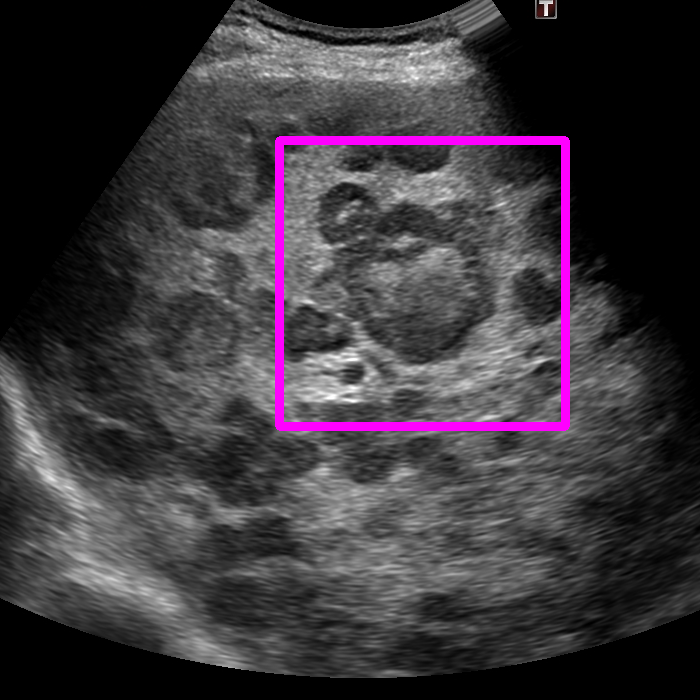
\includegraphics[width=.9\linewidth]{../fig/pseudo.png}
				\caption{アノテーション不足のある診断画像例}
				\label{fig:ex}
			\end{minipage}
		\end{figure}

\footnotetext[1]{今回は\Fref{ex}の様なアノテーションが不足しているものを指す}
\addtocounter{footnote}{1}

	\section{これまでの研究のまとめ}
		\begin{itemize}
			\item データセット
			\begin{itemize}
				\item 国立研究開発法人日本医療研究開発機構(AMED)\footnote{\url{https://www.amed.go.jp/}}が提供している延べ8万人に及ぶ以下のデータが付随している
				\begin{itemize}
					\item 腹部超音波画像,ROI
					\item 年齢,性別
				\end{itemize}
			\end{itemize}
			\begin{figure}[h]
				\centering
				\subfloat[性別毎の画像枚数]{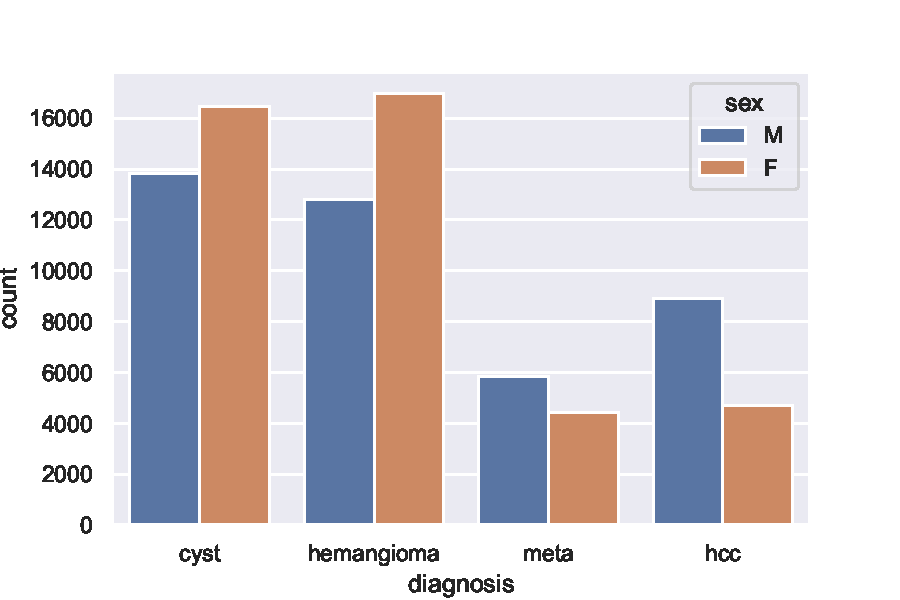
\includegraphics[width=.49\linewidth]{../fig/sex_a.pdf} \label{fig:sex}}
				\subfloat[診断名毎の年齢分布]{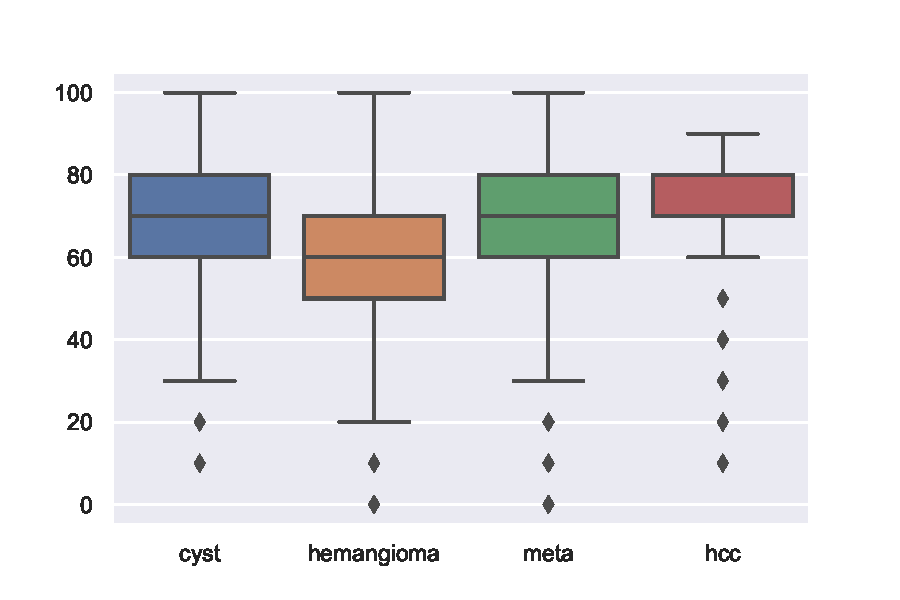
\includegraphics[width=.49\linewidth]{../fig/age_a.pdf} \label{fig:age}}
			\end{figure}
			\begin{itemize}
				\item 性別(\Fref{sex})
				\begin{itemize}
					\item hcc(肝細胞癌)は男性が罹患しやすい
					\item hemangioma(血管腫)は女性が罹患しやすい
				\end{itemize}
				\item 年齢(\Fref{age})
				\begin{itemize}
					\item hcc(肝細胞癌)は比較的高齢者が罹患しやすい
					\item cyst(単純嚢胞),hemangioma(血管腫)の分布にははあまり特徴がない
					\item meta(転移性肝癌)における0歳はラベルミスである可能性が高い
				\end{itemize}
				\begin{figure}[h]
					\centering
					\subfloat[診断名毎の画像サイズ$(h \times w)$の分布]{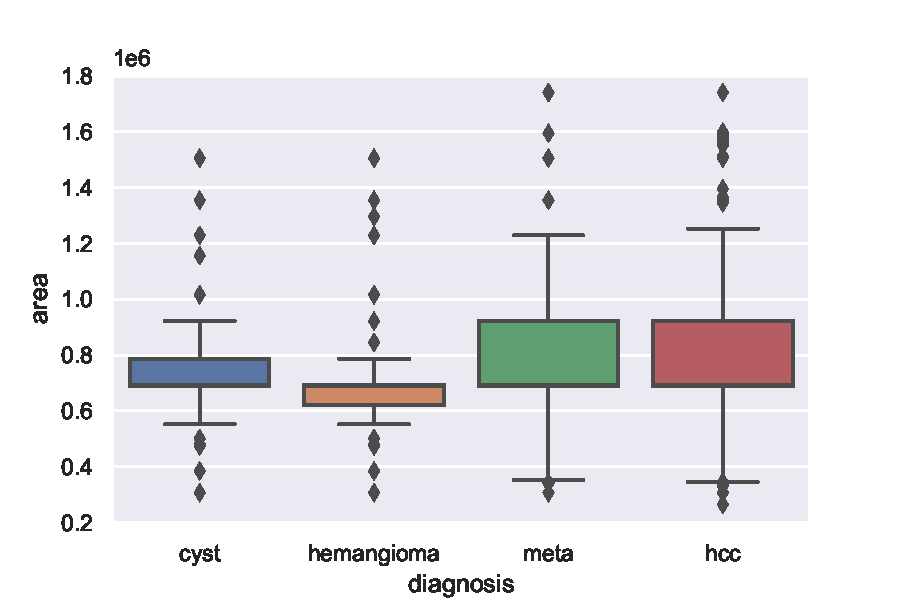
\includegraphics[width=.49\linewidth]{../fig/area_a.pdf} \label{fig:area}}
					\subfloat[診断名毎のbboxの割合]{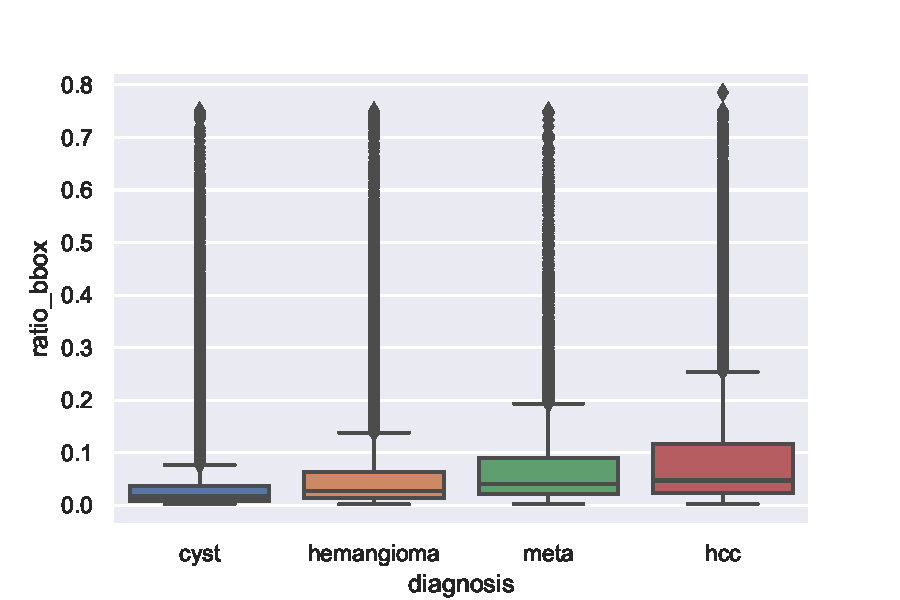
\includegraphics[width=.49\linewidth]{../fig/ratio_bbox_a.pdf} \label{fig:ratio}}
					\caption{データセットに含まれているメタデータの分布}
				\end{figure}
				\item \Fref{area}からhemangioma(血管腫)は比較的画像サイズが統一されていることが読み取れる
				\begin{itemize}
					\item 血管腫においては腫瘍の大きさが血管に依存するためあまり偏りが生じていない?
				\end{itemize}
				\item \Fref{ratio}からcyst(単純嚢胞)は他の診断と比べてbboxの割合が低い($\frac{1}{2}$程度)であることが読み取れる
			\end{itemize}
		\end{itemize}

	\section{前回のGMからの進捗}
		\begin{itemize}
			\item データクレンジングのプロググラムの統合及び改善
			\begin{enumerate}
				\item $400 \times 400$ 以下の画像の除外
				\item Perceptual Hashを利用した類似画像の除外
				\begin{itemize}
					\item 差が2以下であればスキップ
				\end{itemize}
				\item 青色や黄色のスケールの除去
				\begin{itemize}
					\item \Fref{extract}の様にHSV空間で対象の色のある部分のmaskを生成
				\end{itemize}
				\item 使用する画像パスの書き出し
			\end{enumerate}
			\begin{figure}[h]
				\centering
				\subfloat[クレンジング前]{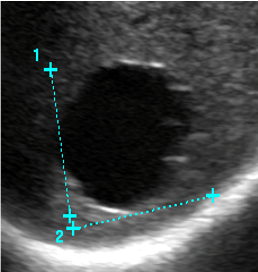
\includegraphics[width=.24\linewidth]{../fig/row.png} \label{fig:row}}
				\subfloat[マスクの生成]{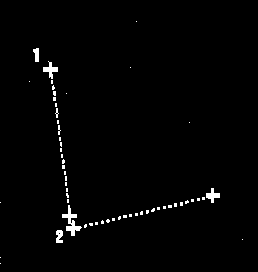
\includegraphics[width=.24\linewidth]{../fig/extract.png} \label{fig:extract}}
				\subfloat[改善前]{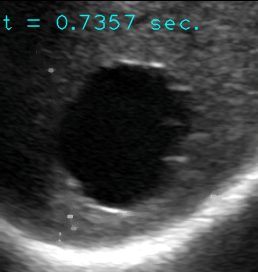
\includegraphics[width=.24\linewidth]{../fig/before.png} \label{fig:before}}
				\subfloat[改善後]{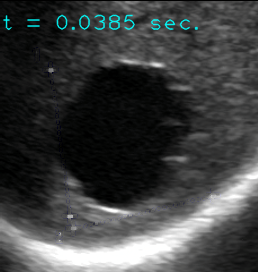
\includegraphics[width=.24\linewidth]{../fig/after.png} \label{fig:after}}
				\caption{データクレンジングを行った結果}
			\end{figure}
			\begin{itemize}
				\item 以前まではデータセット構築として以下を個別に行っていたため時間がかかっていた
				\item 特にデータクレンジングにおいて,\Fref{before}の様に1枚あたり約0.7357秒も必要としていた
				\begin{itemize}
					\item 改善後は約0.0385と\Fref{after}の様に元の精度を保ったまま約20倍高速化
				\end{itemize}
			\end{itemize}
			\begin{minipage}{.64\textwidth}
				\item \Sref{json}における\Lref{json}の様に付随していたメタデータをCOCODatasetの規則に則ったjson形式に
				\begin{itemize}
					\item train,validation,testに分割
				\end{itemize}
			\end{minipage}
			\begin{minipage}{.34\textwidth}
				% \caption{データの個数}
				\label{tab:count}
				\centering
				\begin{tabular}{c|c}
					\hline
					filename & データ数 \\ \hline \hline
					train.json & 67122 \\
					validation.json & 8390 \\
					test.json & 8391 \\
					\hline
				\end{tabular}
			\end{minipage}
			\item \Sref{json}における\Lref{json}の様に付随していたメタデータをCOCODatasetの規則に則ったjson形式に
			\begin{itemize}
				\item COCO形式のデータを扱うために以下をgpgpuの環境にインストール
				\begin{itemize}
					\item \href{https://github.com/cocodataset/cocoapi}{pycocotools}
					\item \href{https://github.com/Jeff-sjtu/CrowdPose}{crowdposetools}
				\end{itemize}
			\end{itemize}
			\item 元の画像から腫瘍の部分の切り出しを行った
			\begin{figure}[ht]
				\centering
				\subfloat[000002.jpg]{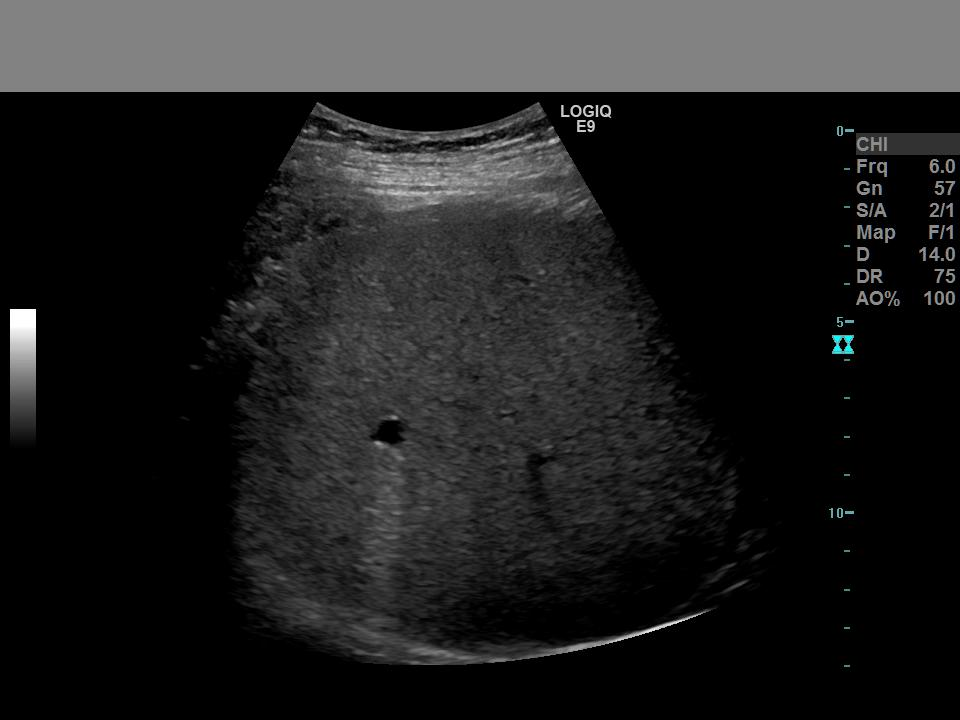
\includegraphics[width=.24\linewidth]{../fig/000002.jpg} \label{fig:02}}
				\subfloat[000019.jpg]{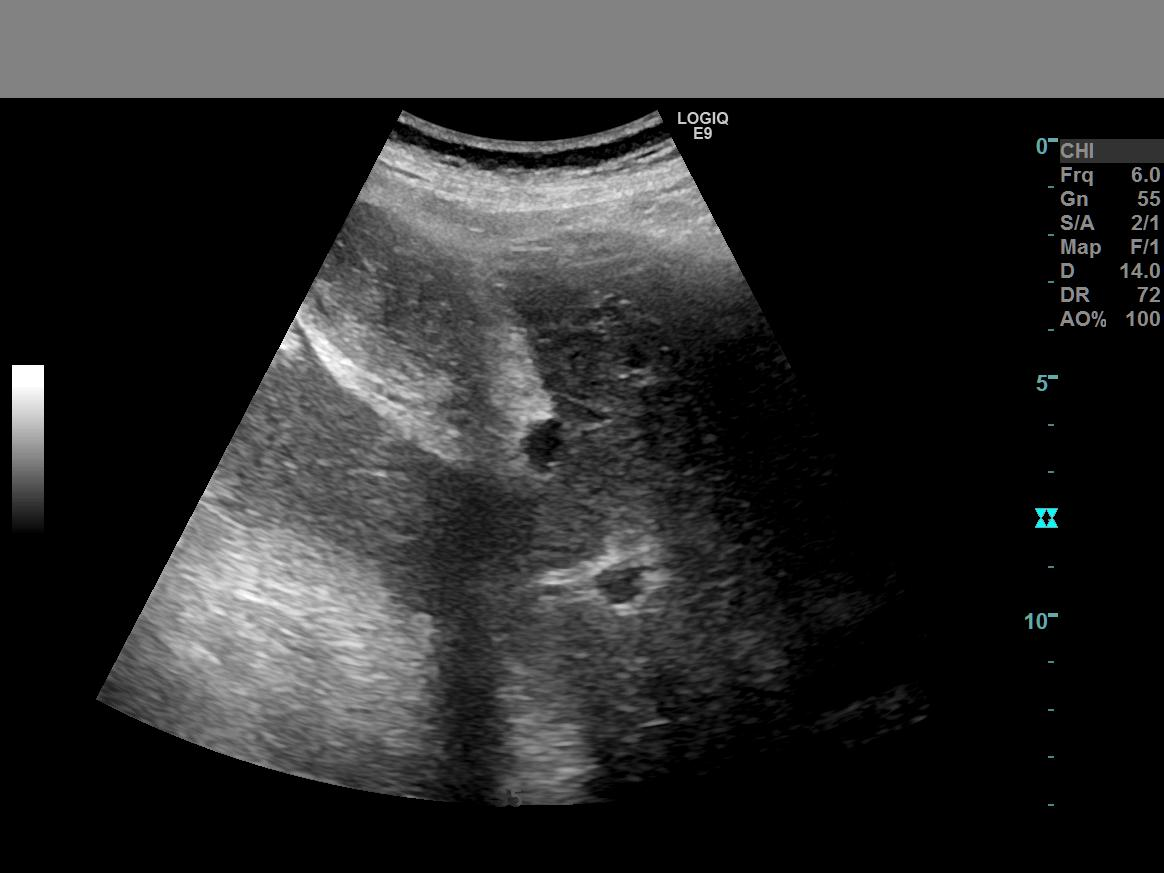
\includegraphics[width=.24\linewidth]{../fig/000019.jpg} \label{fig:19}}
				\subfloat[000027.jpg]{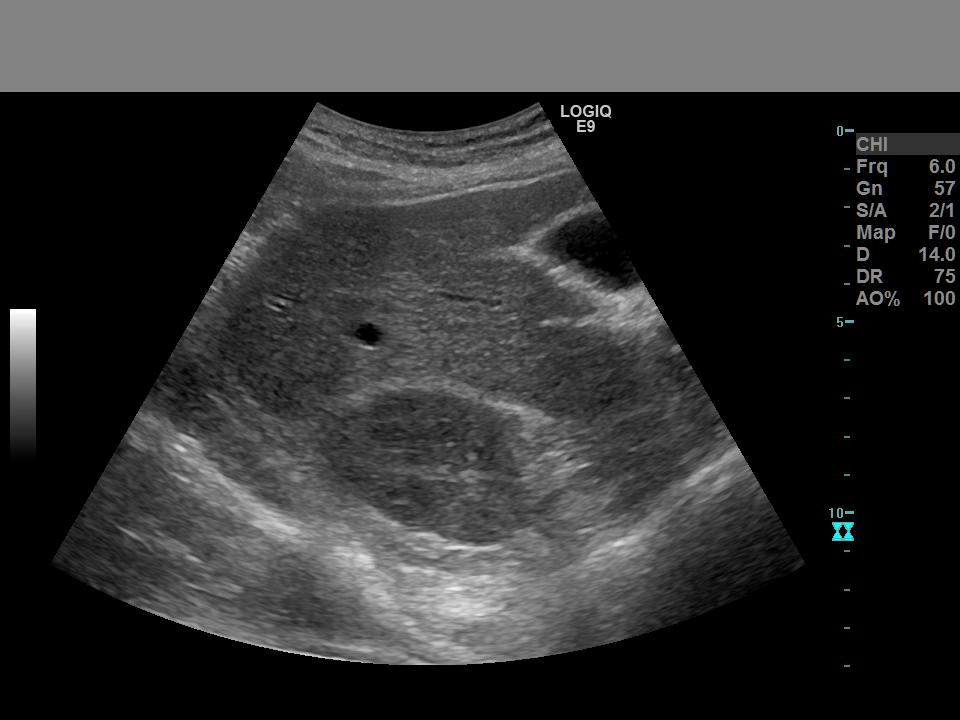
\includegraphics[width=.24\linewidth]{../fig/000027.jpg} \label{fig:27}}
				\subfloat[000040.jpg]{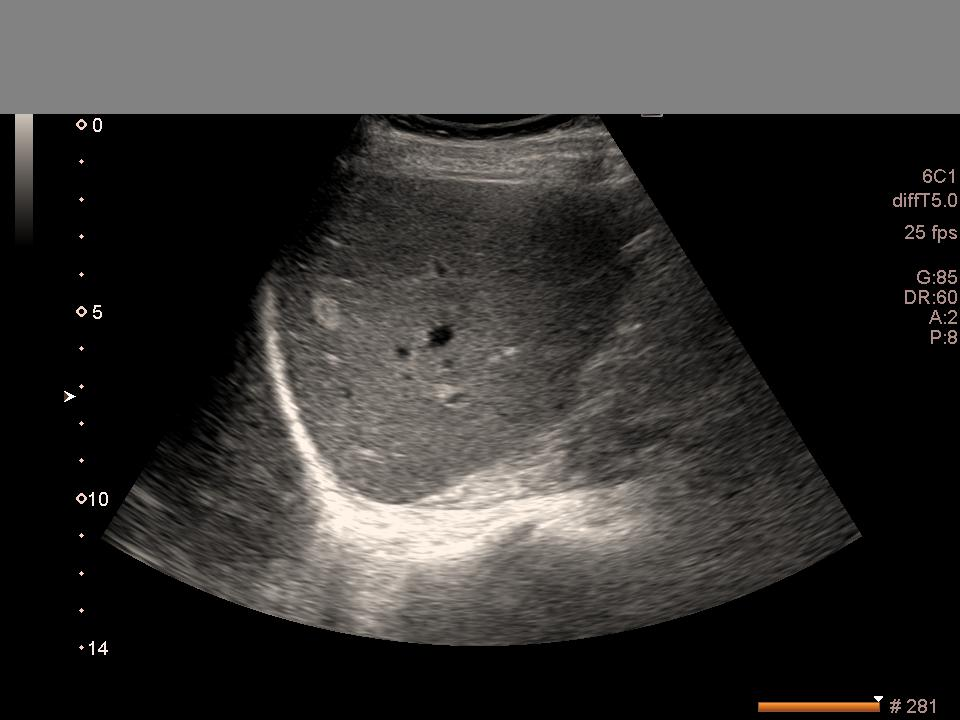
\includegraphics[width=.24\linewidth]{../fig/000040.jpg} \label{fig:40}}
				\caption{元の画像}
			\end{figure}
			\begin{figure}[ht]
				\centering
				\subfloat[000002.jpg]{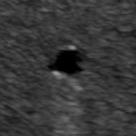
\includegraphics[width=.24\linewidth]{../fig/000002_cut.jpg} \label{fig:02_cut}}
				\subfloat[000019.jpg]{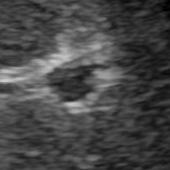
\includegraphics[width=.24\linewidth]{../fig/000019_cut.jpg} \label{fig:19_cut}}
				\subfloat[000027.jpg]{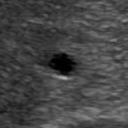
\includegraphics[width=.24\linewidth]{../fig/000027_cut.jpg} \label{fig:27_cut}}
				\subfloat[000040.jpg]{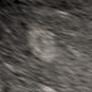
\includegraphics[width=.24\linewidth]{../fig/000040_cut.jpg} \label{fig:40_cut}}
				\caption{腫瘍の切り出しを行った結果}
			\end{figure}
		\end{itemize}

	\section{今後の課題\&スケジュール}
		\begin{itemize}
			\item 11/30まで
			\begin{itemize}
				\item 新規に作成したjson形式のデータでモデルの学習コードを完成させる
			\end{itemize}
			\item できるだけ早めに
			\begin{itemize}
				\item 研究の方向性を決める
				\item Confident Learning \cite{cleanlab} を利用してみる
                \begin{itemize}
                    \item ラベルにノイズが含まれていると予想されるデータセットに対して精度を向上させることができる
                    \item pipでインストールできるcleanlab\footnote{\url{https://github.com/cleanlab/cleanlab}}というライブラリを用いることで簡単に使える
                    \begin{itemize}
                        \item 調べてみたら元はKeras?
                    \end{itemize}
				\end{itemize}
			\end{itemize}
		\end{itemize}

\clearpage

	\appendix
	\def\thesection{付録\Alph{section}}
	\section{jsonファイル}
	\label{sec:json}
	\begin{lstlisting}[language=json, caption={変換後のjsonファイル}, label=lst:json]
{
	"info": {
		"description": "AMED Dataset",
		"url": "https://www.amed.go.jp",
		"version": "1.0",
		"year": 2021,
		"contributor": "Japan Agency for Medical Research and Development",
		"date_created": "2021/10/22"
	},
	"licenses": [{
		"url": "hhttps://www.amed.go.jp",
		"id": 1,
		"name": "Japan Agency for Medical Research and Development"
	}],
	"images": [
		{
			"license": 1,
			"file_name": "000000.jpg",
			"height": 873,
			"width": 1164,
			"id": 0
		},
		...
	],
	"annotations": [
		{
			"iscrowd": 0,
			"image_id": 0,
			"bbox": [317.5,417.5,164.0,164.0],
			"category_id": 1,
			"id": 0,
			"age": 80,
			"sex": 1
		},
		...
	],
	"categories": [
		{
			"supercategory": "cancer",
			"id": 1,
			"name": "cyst"
		},
		...
	]
}
	\end{lstlisting}

	\begin{thebibliography}{9} 
		\bibitem{recognition} Jingdong Wang, Ke Sun, Tianheng Cheng, Borui Jiang, Chaorui Deng, Yang Zhao, Dong Liu, Yadong Mu, Mingkui Tan, Xinggang Wang, Wenyu Liu, and Bin Xiao. \href{https://arxiv.org/pdf/1908.07919.pdf}{Deep High-Resolution Representation Learning for Visual Recognition}, 2020.
		\bibitem{cleanlab} Curtis G. Northcutt, Lu Jiang, and Isaac L. Chuang. \href{https://arxiv.org/pdf/1911.00068.pdf}{Confident Learning: Estimating Uncertainty in Dataset Labels}, 2021.
	\end{thebibliography}
\end{document}
